\documentclass{article}

\usepackage{graphicx}
\graphicspath{ {../pics/} }

% if you need to pass options to natbib, use, e.g.:
% \PassOptionsToPackage{numbers, compress}{natbib}
% before loading nips_2017
%
% to avoid loading the natbib package, add option nonatbib:
% \usepackage[nonatbib]{nips_2017}

\usepackage{nips_2017}
\usepackage{natbib}

% to compile a camera-ready version, add the [final] option, e.g.:
% \usepackage[final]{nips_2017}

\usepackage[utf8]{inputenc} % allow utf-8 input
\usepackage[T1]{fontenc}    % use 8-bit T1 fonts
\usepackage{hyperref}       % hyperlinks
\usepackage{url}            % simple URL typesetting
\usepackage{booktabs}       % professional-quality tables
\usepackage{amsfonts}       % blackboard math symbols
\usepackage{nicefrac}       % compact symbols for 1/2, etc.
\usepackage{microtype}      % microtypography
\usepackage{subcaption}


\title{Relation Extraction for Knowledge Graph and QA System Construction}

% The \author macro works with any number of authors. There are two
% commands used to separate the names and addresses of multiple
% authors: \And and \AND.
%
% Using \And between authors leaves it to LaTeX to determine where to
% break the lines. Using \AND forces a line break at that point. So,
% if LaTeX puts 3 of 4 authors names on the first line, and the last
% on the second line, try using \AND instead of \And before the third
% author name.

\author{
  Zachariah Zhang\\
  Department of Data Science\\
  New York University\\
  New York, NY 10012 \\
  \texttt{zz1409@nyu.edu} \\
  \And
  Lizi Chen\\
  Department of Computer Science\\
  New York University\\
  New York, NY 10012 \\
  \texttt{lc3397@nyu.edu} \\
  \And
  Guangyu Zhang\\
  Department of Computer Science\\
  New York University\\
  New York, NY 10012 \\
  \texttt{guangyu.zhang@nyu.edu} \\
  %% examples of more authors
  %% \And
  %% Coauthor \\
  %% Affiliation \\
  %% Address \\
  %% \texttt{email} \\
  %% \AND
  %% Coauthor \\
  %% Affiliation \\
  %% Address \\
  %% \texttt{email} \\
  %% \And
  %% Coauthor \\
  %% Affiliation \\
  %% Address \\
  %% \texttt{email} \\
  %% \And
  %% Coauthor \\
  %% Affiliation \\
  %% Address \\
  %% \texttt{email} \\
}

\begin{document}
% \nipsfinalcopy is no longer used

\maketitle

\begin{abstract}
	The ultimate goal of this project is to build a Question-Answering (QA) application based on generated Knowledge Graph (KG) from raw text data. For the following two parts, we will focus on part 1, and will explore part 2 if time permitted.
	 \begin{enumerate}
	 	\item Knowledge Graph construction from raw text data;
	 	\item \emph{(Tentative, will do only if time permits)} Question-Answering application on top of the graph. May use it for metrics and evaluation.
 	\end{enumerate}
 
	This is a joint project for the two courses: 2/3 authors have enrolled in the "Statistical NLP" course, and 2/3 authors have enrolled in the "Inference and Representation" .
\end{abstract}


\section{Problem to address}

	Natural language text is typically very unstructured which makes many different machine learning applications difficult. A knowledge graph can be used to model the relationships of different entities in a body of text. These graphs create a lot of value for other machine learning applications such as question answering and reading comprehension. 
	
	In recent years, deep learning has seen boom in popularity for nlp problems with its ability to model complicated and ambiguous text. Traditionally, people have adapted statistical methods, e.g. POS-tags, named entity tags, to extract entities relations, and reached an precision of 67.6%.\\
	In the work we will do a review of the literature around deep learning methods for knowledge graph extraction. 
	
	Based on revising recent papers, we will create program which consumes data into knowledge graph based on some available dataset as listed in the next sections. We will tweak the parameters, analyze the existing models, and further improve on selective ones. We may tentatively provide a Question-Answering testing application for graph demonstration and evaluation; however, given the amount of work and limited time in the remaining semester, we will only work on this part when time permits.
  
\section{Datasets}
	
	\paragraph{Freebase} This data set has been massively used in many knowledge graph publications.
	
	\paragraph{Nell-995} So is this one, which has been used in the Reinforcement Learning paper by Wenhan et al., 2017.
	
	\paragraph{Dataset used in \citet{Riedel2010}} This dataset was formed by aligning Freebase relations with the New York Times corpus (NYT). Entity mentions were found in the documents using the Stanford named entity tagger, and are further matched to the names of Freebase entities.

\section{Algorithms}

\subsection{Distant supervision}
	Relation extraction plays a key role in knowledge graph. Traditionally, supervised techniques are adopted for non deep learning methods, but requires intensive human labors of annotation. \citet{Mintz:2009:DSR:1690219.1690287} proposed a distant supervision method of automatically generating training data, via aligning documents with known knowledge base (Freebase). They have extracted lexical (e.g. sequence of words, POS tags) and syntactic (dependency parser) features, and performed named entity tagging by Stanford four-class named entity tagger \citet{Finkel:2005:INI:1219840.1219885}. Their model is reported to extract 10,000 instances of 102 relations at a precision of $67.6\%$.
	
	\citet{Mintz:2009:DSR:1690219.1690287} has an assumption such that if two entities participate in a relation, any sentence that contain those two entities might express that relation, while in reality may result to non-trivial noises. \citet{Riedel2010} alleviates noises via deciding whether two entities are related and also mentioned in a given sentence, and then applying "constraint-driven semi-supervision" to train

\subsection{Deep learning tsunami in KG}

\subsubsection{PCNN with attention mechanism}
	We will compare work developed in several different deep learning publications. We will focus on the basic CNN model (Zeng et al 2014), Piecewise CNN (Zeng et al 2015), CNN with multiple kernels (Thien and Grishman et al 2015), as well as the use of attention (Lin et al 2016). Compare the tradeoffs between these model architectures and compare with non-deep learning baselines. \citet{DBLP:conf/acl/LinSLLS16}
	
	Yankai Lin et al 2016 improved the Distant supervised relation extraction method with additional attention mechanism over its previous work. The improved version has CNN for semantic feature extraction and a sentence-level attention for the purpose of reducing wrong labeling weights. 
	
	\begin{figure}[h!]
		\centering
		\begin{subfigure}[b]{0.2\linewidth}
			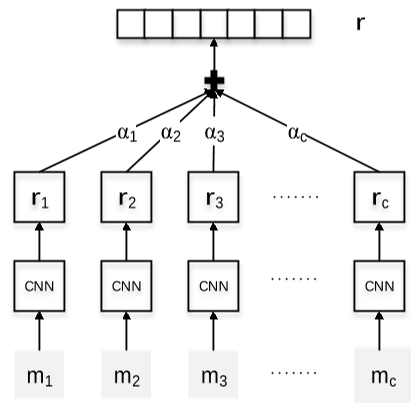
\includegraphics[width=\linewidth]{figure1.png}
			\caption{The architecture of sentence-level attention-based CNN. Used in Yankai Lin et al 2016}
		\end{subfigure}
		\begin{subfigure}[b]{0.2\linewidth}
			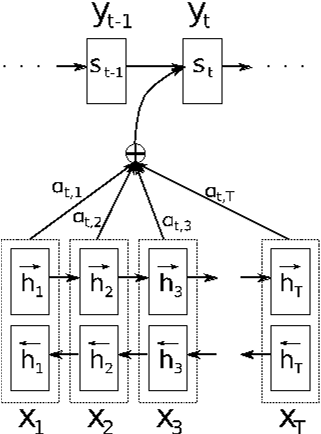
\includegraphics[width=\linewidth]{attention-method-1.png}
			\caption{Classical attention mechanism used in Dzmitry arXiv:1409.0473}
		\end{subfigure}
		\caption{Comparison between two attentions.}
		\label{fig:compare}
	\end{figure}
	
	\paragraph{Input Vector Representation}
	There are many paradigms of word embedding; converting human-readable vocabularies into numbers that can be processed by machine. Two major approaches from the past several years are the Frequency based Embedding and Prediction based Embedding. 
	
	There are two embedding steps done for the input vector representation in this paper. One is word embedding, which aims to capture syntactic and semantic meanings of the words. The other one is based on the assumption that words that close to the target entities are usually informative to determine the relation between entities. Thus, the result vector is a concatenation of the word embedding matrix and the position embedding one. The result vector:
	\[w_i \in \mathbb{R}^d(d = d^a + d^b \times 2) \]
	where \(d^a\) is the dimension of the word embedding and \(d^b\) is the dimension of position embedding.
	
	\begin{figure}[h!]
		\centering	
		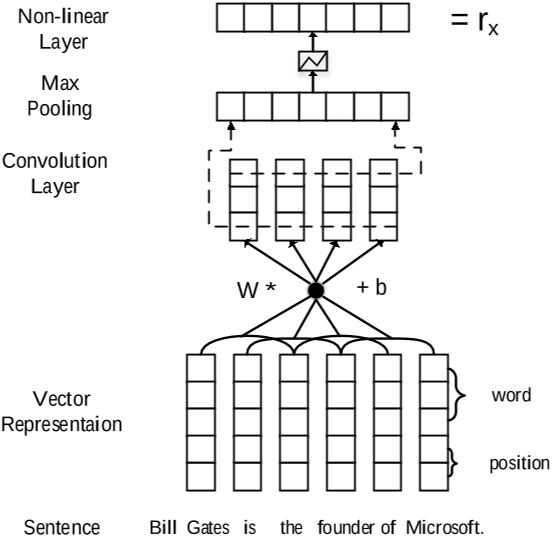
\includegraphics[scale=0.2]{figure2.png}
		\caption{The architecture of CNN/PCNN used for sentence encoder}
	\end{figure}	

	\paragraph{Convolution, Max-pooling, Zero-paddings, and Non-Linear Layers}
	Due to the fact that vector representation from previous step has all different size, max-pooling is required to obtain a fixed-sized vector for the input sentence.
	
	\paragraph{Selective Attention over Instances}
	One of the core innovative part from this paper, which makes the result stood out from past works, is the attention mechanism for all entities and providing various weights to reduce wrong entities label. For each previous layer, attention attribute is added as:
	\[a_i = \frac{\exp(e_i)}{\displaystyle\sum_{k} \exp(e_k)}\]
	where \(e_i = x_i A r\) \\
	\(A\) is a matrix, \(r\) represents the relation in matrix, which is mentioned in the previous paper as well. Therefore, \(e_i\) means the matching between the sentence and entities.
	
	The final result conditional probability can be represented as the following through a softmax layer:
	\[p(r|S, \theta) = \frac{\exp(o_r)}{\displaystyle\sum_{k=1}^{n_r} \exp(o_k)}\]

	\(n_r\) = total number of relations \\
	\(o\) = the final output of the neural network, which corresponds to the scores associated to all relation types. \\
	\(\theta\) = the parameter of this model \\
	\[o = Ms + d\]	

	Therefore, the objective function using cross-entropy for the training is:
	\[J(\theta) = \displaystyle\sum_{i=1}^{s} \log(p(r_i|S_i, \theta)) \]
	The paper uses mini-batch chosen randomly from the training set as the result converge.
	
\subsection{Reinforcement learning}	
	\textit{This part of investigation has yet to be completed.} \\
	Wenhan et al., 2017 have studied the problem of learning to reason in knowledge graphs (KGs) specifically in large scale. A novel reinforcement learning framework for learning multi-hop relational paths is introduced: A policy-based agent with continuous states based on knowledge graph embeddings, which reasons in a KG vector-space by sampling the most promising relation to extend its path. In contrast to prior work, such approach includes a reward function that takes the accuracy, diversity, and efficiency into consideration. Experimentally, results from this paper show that the proposed method outperforms a path-ranking based algorithm and knowledge graph embedding methods on Freebase and Never-Ending Language Learning datasets.
	
	\textit{Further investigation details will be added here.} \\

\subsection{General optimization methods}
	The papers that we have investigated adopts general stochastic gradient descent (SGD) to minimize objective function.
	Dropout layer (Srivastava et al., 2014) is implemented on the output layer to prevent overfitting.

\section{Evaluation Metric}
	We will evaluate each model on precision, recall, and F score to be consistent with the literature.
  
\section{Questions}


\medskip

\bibliography{proposal}
\bibliographystyle{achemso}

\small


\end{document}